\chapter{Implementación}

Se ha desarrollado un recomendador básico utilizando el lenguaje de programación \texttt{Python} y la base de datos \texttt{Movie Lens}.

\bigskip
En cuanto al desarrollo del algoritmos k-NN se han desarrollado siguiendo los ejemplos de la correlación de Pearson del temario de la asignatura puesto que indica que es la mas óptima.

\[ sim(u,v) = \frac{\sum(r(u,i)-\bar{r}(u))(r(v,i)-\bar{r}(v))}{\sqrt{\sum(r(u,i)-\bar{r}(u))^2}\sqrt{\sum(r(v,i)-\bar{r}(v))^2}} \]
Donde $ r(u,i) $ es la valoración del usuario \textit{u} a la película \textit{i} y $ \bar{r}(u) $ la valoración media del usuario \textit{u}.

\bigskip
Para \textit{predecir} la valoración que le daríamos al resto de las películas hemos usado el siguiente algoritmo:

\[ \hat{r}(u,i) = \bar{r}(u) + \frac{sim(u,v)(r(v,i)-\bar{r}(v))}{\sum|sim(u,v)|} \]

Donde $ r(v,i) $ es la valoración del usuario \textit{v} a la película \textit{i}, $ \bar{r}(u) $ la valoración media del usuario \textit{u} y $ sim(u,v) $ la similitud entre los usuarios \textit{u} y \textit{v} calculada anteriormente.

\bigskip
Por último se han seleccionado las \textit{n} películas con mayor valoración siempre y cuando dicha valoración sea superior a 4 estrellas.

\bigskip
Como curiosidad hay que notar que el algoritmo recomienda algunas películas por encima de las 5 estrellas en base a la afinidad con otros vecinos. Se ha dejado así porque evidentemente una valoración por encima de 5 significa una mejor recomendación aunque en el código tenemos la posibilidad de limitar las valoraciones a 5 estrellas.

\bigskip
Para mejorar la interacción del programa se le han agregado colores a la salida en pantalla, además se permiten dos modos, el modo interactivo que iría preguntado la valoración que le queremos asignar a cada una de las películas seleccionada aleatoriamente así como el modo automático que asignaría las valoraciones de las películas del usuario de forma aleatoria.

\begin{figure}
\centering
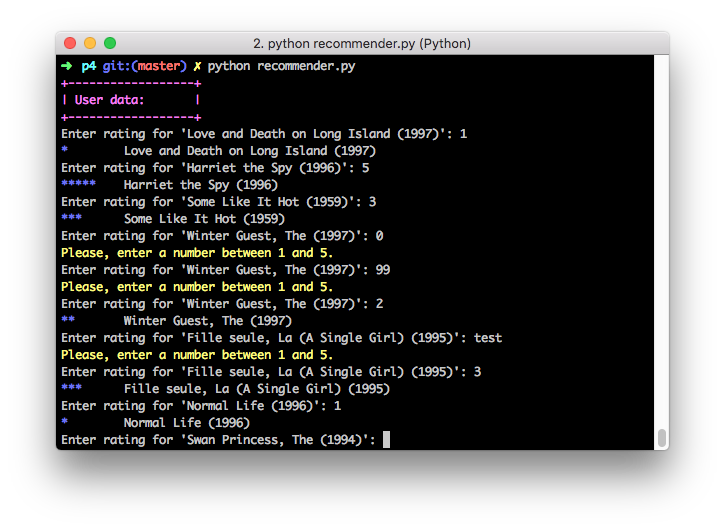
\includegraphics[width=1.1\textwidth]{../images/interactive.png}
\caption{Ejecución interactiva}
\end{figure}

\bigskip
Se ha hecho especial detalle en controlar las posibles excepciones del usuario a la hora de introducir las valoraciones, también se ha controlado la codificación de los archivos para no representar caracteres extraños.

\bigskip
Aunque se podría haber optimizado la ejecución de este programa usando la librería \texttt{Numpy} no ha sido necesario puesto que el volumen de datos es relativamente pequeño y se ha optado por usar los propios diccionarios de \texttt{Python}.

\begin{figure}
\centering
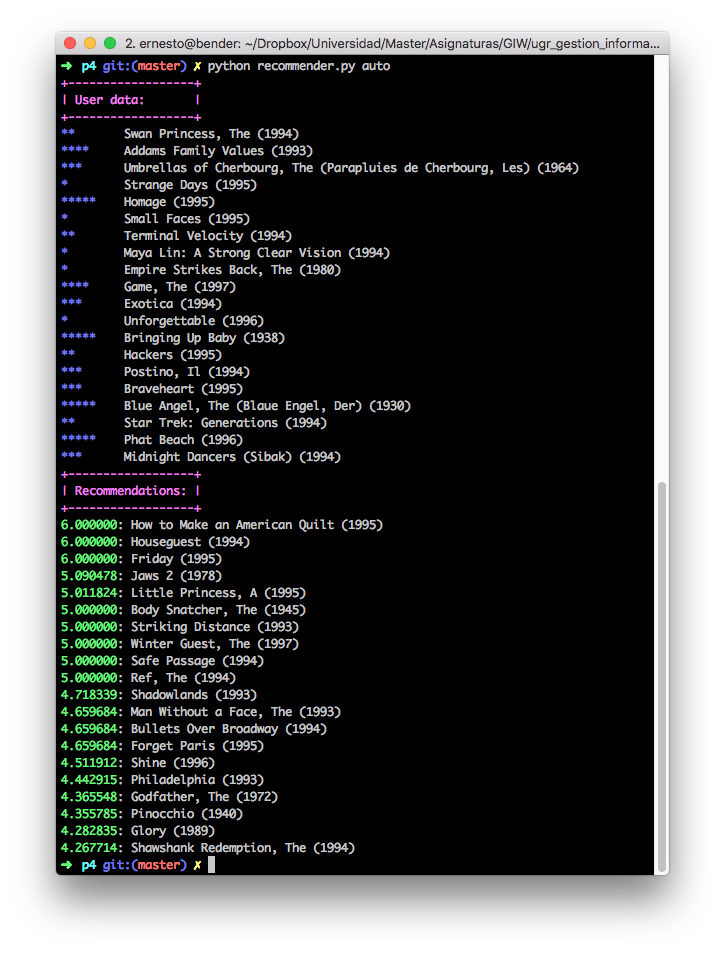
\includegraphics[width=1.0\textwidth]{../images/automatic.png}
\caption{Ejecución automática}
\end{figure}
